\subsection{滤子化集合上定义的实值函数}

命题 1. 设 \(f\) 与 \(g\) 是定义在集合 \(\mathbf{X}\) （它由滤子 \(\mathfrak{F}\) 滤子化）上的两个实值函数。若 \(\lim_{\mathfrak{F}} f\) 与 \(\lim_{\mathfrak{F}} g\) 存在，且对每个子集 \(\mathbf{A} \in \mathfrak{F}\) 存在 \(x \in \mathbf{A}\) 使得 \(f(x) \leqslant g(x)\) ，则我们有 \(\lim_{\mathfrak{F}} f \leqslant \lim_{\mathfrak{F}} g\) 。

为证明这一结果，我们将证明下述等价的命题：

命题 2. 设 \(f\) 与 \(g\) 是定义在集合 \(X\) （它由滤子 \(\mathfrak{F}\) 滤子化）上的两个实值函数。若 \(\lim_{\mathfrak{F}} f\) 与 \(\lim_{\mathfrak{F}} g\) 存在，且 \(\lim_{\mathfrak{F}} f > \lim_{\mathfrak{F}} g\) ，则存在一个集 \(A \in \mathfrak{F}\) ，使得 \(f(x) > g(x)\) 对一切 \(x \in A\) 成立。

设 \(a = \lim_{\mathfrak{F}} f\) ，设 \(b = \lim_{\mathfrak{F}} g\) ，并设 \(c\) 满足 \(b < c < a\) 。区间 \(]c, +\infty]\) （属于 \(\overline{\mathbf{R}}\) ）（相应地，\([-\infty, c[)\) ）是 \(a\) （相应地，\(b\) ）的邻域；因此存在一个集 \(M \in \mathfrak{F}\) （相应地，一个集 \(N \in \mathfrak{F}\) ），使得 \(f(x) > c\) 对一切 \(x \in M\) 成立{[}相应地，\(g(x) < c\) 对一切 \(x \in N\) 成立{]}。集 \(A = M \cap N\) 属于 \(\mathfrak{F}\) ，且 \(f(x) > c > g(x)\) 对一切 \(x \in A\) 成立。

作为命题 1 的一个特例，我们有下述定理：

定理 1（不等式延拓原理）. 设 \(f\) 与 \(g\) 是定义在集合 \(\mathbf{X}\) （它由滤子 \(\mathfrak{F}\) 滤子化）上的两个实值函数。若 \(\lim_{\mathfrak{F}} f\) 与 \(\lim_{\mathfrak{F}} g\) 存在，且 \(f \leqslant g\) ，则 \(\lim_{\mathfrak{F}} f \leqslant \lim_{\mathfrak{F}} g\) 。

\pandocbounded{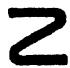
\includegraphics[keepaspectratio]{images/part002_67e89114.jpg}}

注. 特别地，若 \(f(x) < g(x)\) 对一切 \(x \in X\) 成立（或者只对滤子 \(\overline{\mathbf{R}}\) 的某一个集中的各点成立），则由定理 1 可以推出 \(\lim_{\mathfrak{F}} f \leqslant \lim_{\mathfrak{F}} g\) ；但我们不能推出严格不等式 \(\lim_{\mathfrak{F}} f < \lim_{\mathfrak{F}} g\) 。例如，取 \(X\) 为自然数集 \(N\) ，赋以 Fréchet 滤子，且设 \(f(n) = 0\) ，\(g(n) = 1/n\) ，则 \(f(n) < g(n)\) 对一切 \(n\) 成立，但 \(\lim_{n \to \infty} f(n) = \lim_{n \to \infty} f(n) = 0\) 。因此，在严格不等式中过渡到极限时，严格性会丢失。

定理 2（单调极限定理）. 设 X 是一个有序集，A 是 X 的一个有向子集 (*)。每个定义在 A 上的单调实值函数 f 关于 A 都有极限（第一章，§ 7，第 3 节）；若 f 递增（相应地，递减），则此极限等于集 \(f(A) \subset \overline{\mathbf{R}}\) 的上确界（相应地，下确界）。

例如设 \(f\) 递增，并令 \(a = \sup f(A)\) 。若 \(a = -\infty\) ，定理是平凡的。若 \(a > -\infty\) ，则对每个 \(b < a\) 存在 \(x \in A\) 使得 \(b < f(x) \leqslant a\) ；于是，若 \(S_x\) 是 \(A\) 的相对于 \(x\) 的截面（即所有 \(y \geqslant x\) 所成之集，参看第一章，§ 6，第 3 节），则 \(f(S_x)\) 含于 \(]b, +\infty]\) （它是 \(a\) 的一个邻域）之中，定理得证。若 \(f\) 递减，证明类似。

推论. 定义在有序集 X 的有向子集 A 上的递增（相应地，递减）实值函数，关于 A 有有限极限的充分必要条件是它在 A 中上有界（相应地，下有界）。

若把定理 2 应用于 \(\mathbf{A} = \mathbf{X} = \mathbf{N}\) （按关系 \(\leqslant\) 定序）的情形，就得到下述命题：

命题 3. 每个实数单调序列在 R 中有极限。特别地，由有限数组成的递增（相应地，递减）序列，当其上有界（相应地，下有界）时收敛于一个有限实数，否则收敛于 +∞（相应地，-∞）。例如，正整数序列收敛于 +∞。

这一事实正是用记号 \(\lim_{n\to \infty}u_n\) 表示序列极限的由来（第一章，§ 7，第 3 节）。

同样，每个严格递增的整数序列 \((p_n)\) 收敛于 \(+\infty\) ；因为由归纳法可见，\(p_n \geqslant p_0 + n\) 对一切 \(n\) 成立。

